% ======================================================================================
% ======================================================================================
% ====================================================================================== 

\newcommand\figIsbiTemplateFigure{
    \begin{figure}[htb]
    
    \begin{minipage}[b]{1.0\linewidth}
      \centering
      \centerline{\includegraphics[width=8.5cm]{example-image}}
    %  \vspace{2.0cm}
      \centerline{(a) Result 1}\medskip
    \end{minipage}
    %
    \begin{minipage}[b]{.48\linewidth}
      \centering
      \centerline{\includegraphics[width=4.0cm]{example-image}}
    %  \vspace{1.5cm}
      \centerline{(b) Results 3}\medskip
    \end{minipage}
    \hfill
    \begin{minipage}[b]{0.48\linewidth}
      \centering
      \centerline{\includegraphics[width=4.0cm]{example-image}}
    %  \vspace{1.5cm}
      \centerline{(c) Result 4}\medskip
    \end{minipage}
    %
    \caption{Example of placing a figure with experimental results.}
    \label{fig:isbi_template}
    %
    \end{figure}
}

% ======================================================================================
% ======================================================================================
% ======================================================================================

\newcommand\figQualitative{
\begin{figure*}[tb]
    \centering
    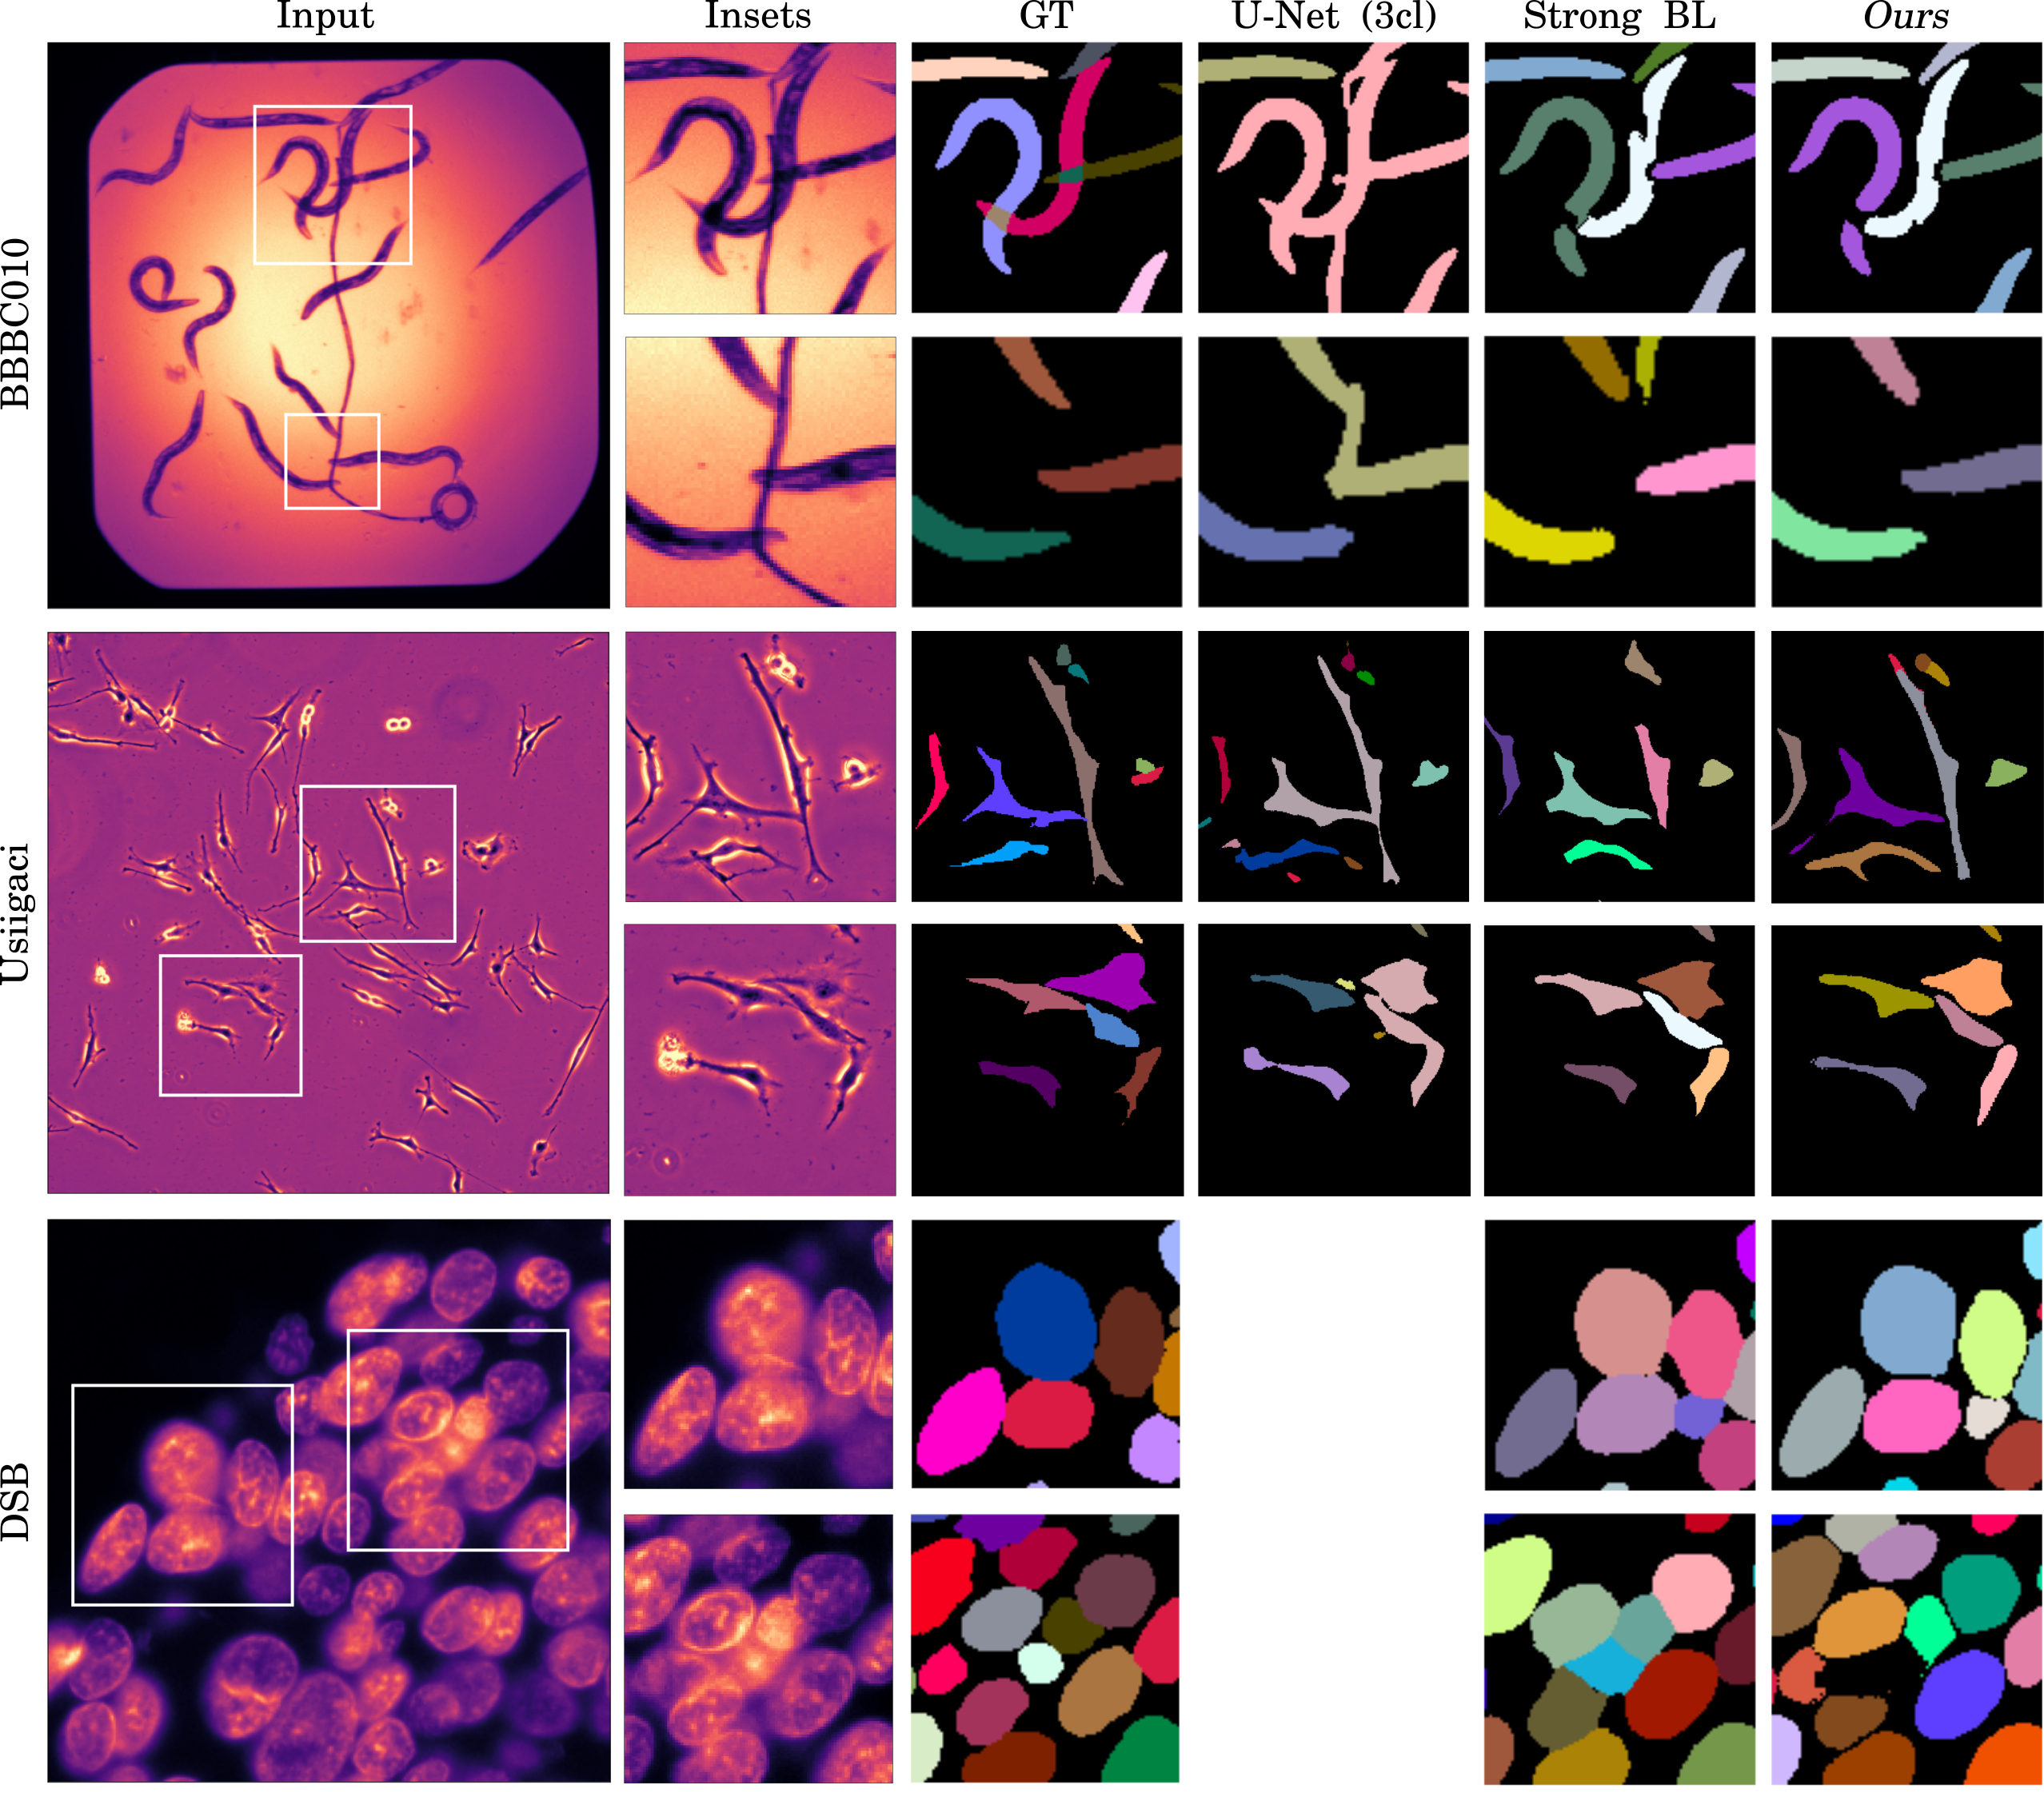
\includegraphics[width=.9\textwidth,trim=0 600 0 0, clip]{figs/qualitative_Template2.png}
    
    \caption{\small
    Qualitative results of \EmbedSeg and two baselines on one representative image of the BBBC010 and Usiigaci dataset.
    Columns show one input image, zoomed insets, ground truth labels (GT), and instance segmentation results by the 3-class U-Net baseline, the best performing competing baseline, and our results using \EmbedSeg. Note that each segmented instance is shown in a random but unique color.
    }
    \label{fig:qualitative}
\end{figure*}
}